% =============================================================================
% Lecture 06: Forecast Evaluation
% BSAD 8310: Business Forecasting
% University of Nebraska at Omaha
% =============================================================================

\documentclass[aspectratio=169, 11pt]{beamer}

% =============================================================================
% header.tex — BSAD 8310: Business Forecasting
% University of Nebraska at Omaha
% Beamer theme: UNO-branded, clean, professional
% =============================================================================

% ----------------------------- BEAMER THEME ----------------------------------
\usetheme{default}
\useinnertheme{rectangles}

% ----------------------------- UNO COLOR PALETTE -----------------------------
\definecolor{unoblue}{HTML}{005CA9}
\definecolor{unored}{HTML}{E41C38}
\definecolor{unogray}{HTML}{525252}
\definecolor{unogreen}{HTML}{15803d}
\definecolor{unolightblue}{HTML}{E8F0FA}
\definecolor{unolightred}{HTML}{FDECEA}
\definecolor{unolightgreen}{HTML}{F0FAF4}
\definecolor{unowhite}{HTML}{FFFFFF}

% Apply UNO colors to Beamer structure
\setbeamercolor{structure}{fg=unoblue}
\setbeamercolor{palette primary}{bg=unoblue, fg=white}
\setbeamercolor{palette secondary}{bg=unoblue!80!black, fg=white}
\setbeamercolor{palette tertiary}{bg=unoblue!60!black, fg=white}
\setbeamercolor{frametitle}{bg=unoblue, fg=white}
\setbeamercolor{frametitle right}{bg=unoblue!80!black}
\setbeamercolor{title}{fg=unoblue}
\setbeamercolor{subtitle}{fg=unogray}
\setbeamercolor{author in head/foot}{bg=unoblue, fg=white}
\setbeamercolor{title in head/foot}{bg=unoblue!80, fg=white}
\setbeamercolor{date in head/foot}{bg=unoblue!60, fg=white}
\setbeamercolor{page number in head/foot}{bg=unoblue!60, fg=white}
\setbeamercolor{block title}{bg=unoblue, fg=white}
\setbeamercolor{block body}{bg=unolightblue}
\setbeamercolor{block title alerted}{bg=unored, fg=white}
\setbeamercolor{block body alerted}{bg=unolightred}
\setbeamercolor{block title example}{bg=unogreen, fg=white}
\setbeamercolor{block body example}{bg=unolightgreen}
\setbeamercolor{itemize item}{fg=unoblue}
\setbeamercolor{itemize subitem}{fg=unored}
\setbeamercolor{enumerate item}{fg=unoblue}
\setbeamercolor{enumerate subitem}{fg=unored}
\setbeamercolor{alerted text}{fg=unored}

% ----------------------------- FONTS -----------------------------------------
\usefonttheme{professionalfonts}
\usefonttheme[onlymath]{serif}       % serif math; sans-serif text
\setbeamerfont{frametitle}{size=\large, series=\bfseries}
\setbeamerfont{title}{size=\LARGE, series=\bfseries}
\setbeamerfont{subtitle}{size=\large}
\setbeamerfont{block title}{size=\normalsize, series=\bfseries}
\setbeamerfont{footline}{size=\tiny}

% ----------------------------- LAYOUT ----------------------------------------
\setbeamersize{text margin left=0.5cm, text margin right=0.5cm}
\setbeamertemplate{navigation symbols}{}   % remove navigation buttons
\setbeamertemplate{itemize items}[circle]
\setbeamertemplate{enumerate items}[default]

% Custom footline: [Course] [Title] [Page/Total]
\setbeamertemplate{footline}{%
  \leavevmode%
  \hbox{%
    \begin{beamercolorbox}[wd=.33\paperwidth, ht=2.5ex, dp=1ex, left, leftskip=4pt]
      {author in head/foot}%
      \usebeamerfont{author in head/foot}\insertshortauthor
    \end{beamercolorbox}%
    \begin{beamercolorbox}[wd=.34\paperwidth, ht=2.5ex, dp=1ex, center]
      {title in head/foot}%
      \usebeamerfont{title in head/foot}\insertshorttitle
    \end{beamercolorbox}%
    \begin{beamercolorbox}[wd=.33\paperwidth, ht=2.5ex, dp=1ex, right, rightskip=4pt]
      {date in head/foot}%
      \usebeamerfont{date in head/foot}%
      \insertframenumber{} / \inserttotalframenumber
    \end{beamercolorbox}%
  }%
  \vskip0pt%
}

% Frametitle with thin accent line
\setbeamertemplate{frametitle}{%
  \vskip0.1cm
  \insertframetitle
  \vskip0.05cm
  \color{unored}\rule{\textwidth}{0.5pt}
}

% Title page
\setbeamertemplate{title page}{%
  \vfill
  \begin{center}
    {\color{unoblue}\rule{\textwidth}{2pt}}\\[0.3cm]
    {\usebeamerfont{title}\usebeamercolor[fg]{title}\inserttitle}\\[0.2cm]
    {\usebeamerfont{subtitle}\usebeamercolor[fg]{subtitle}\insertsubtitle}\\[0.3cm]
    {\color{unored}\rule{\textwidth}{0.5pt}}\\[0.4cm]
    {\small\insertauthor}\\[0.1cm]
    {\small\insertinstitute}\\[0.1cm]
    {\small\insertdate}
  \end{center}
  \vfill
}

% ----------------------------- PACKAGES --------------------------------------

% Math
\usepackage{amsmath}
\usepackage{amssymb}
\usepackage{mathtools}
\usepackage{bm}                    % bold math symbols

% Graphics & color
\usepackage{graphicx}
\usepackage{xcolor}
\usepackage{tikz}
\usetikzlibrary{arrows.meta, positioning, shapes, fit, backgrounds, calc}
\usepackage{pgfplots}
\pgfplotsset{compat=1.18}

% Tables
\usepackage{booktabs}
\usepackage{array}
\usepackage{multirow}
\usepackage{tabularx}

% Typography
\usepackage{microtype}
\usepackage{url}
\usepackage{hyperref}
\hypersetup{colorlinks=true, linkcolor=unoblue, urlcolor=unoblue, citecolor=unogray}

% Code listings (no shell-escape required)
\usepackage{listings}
\lstset{
  language=Python,
  basicstyle=\ttfamily\footnotesize,
  keywordstyle=\color{unoblue}\bfseries,
  stringstyle=\color{unogreen},
  commentstyle=\color{unogray}\itshape,
  numberstyle=\tiny\color{unogray},
  breaklines=true,
  showstringspaces=false,
  frame=single,
  rulecolor=\color{unogray!40},
  backgroundcolor=\color{unogray!5},
  xleftmargin=0.5em,
  xrightmargin=0.5em,
}

% Bibliography
\usepackage[backend=bibtex, style=authoryear, maxcitenames=2]{biblatex}
\addbibresource{../Bibliography_base.bib}

% Colored text helpers
\usepackage{tcolorbox}
\tcbuselibrary{skins, breakable, listingsutf8}

% ----------------------------- CUSTOM ENVIRONMENTS ---------------------------

% keybox: UNO-blue background — for key results, formulas, takeaways
\newtcolorbox{keybox}{
  enhanced,
  colback=unoblue,
  colframe=unoblue!80!black,
  coltitle=white,
  coltext=white,
  fonttitle=\bfseries,
  boxrule=0pt,
  arc=3pt,
  left=4pt, right=4pt, top=3pt, bottom=3pt,
}

% definitionbox: blue left-rule with title — for formal definitions
\newtcolorbox{definitionbox}[1]{
  enhanced,
  title={#1},
  colback=unolightblue,
  colframe=unoblue,
  coltitle=unoblue,
  fonttitle=\bfseries,
  boxrule=0pt,
  leftrule=3pt,
  arc=0pt,
  left=4pt, right=4pt, top=3pt, bottom=3pt,
}

% warningbox: red-accent — for pitfalls, assumption violations, common errors
\newtcolorbox{warningbox}{
  enhanced,
  colback=unolightred,
  colframe=unored,
  coltitle=white,
  fonttitle=\bfseries,
  boxrule=0pt,
  leftrule=3pt,
  arc=0pt,
  left=4pt, right=4pt, top=3pt, bottom=3pt,
}

% examplebox: green-accent with title — for worked examples, business applications
\newtcolorbox{examplebox}[1]{
  enhanced,
  title={#1},
  colback=unolightgreen,
  colframe=unogreen,
  coltitle=unogreen,
  fonttitle=\bfseries,
  boxrule=0pt,
  leftrule=3pt,
  arc=0pt,
  left=4pt, right=4pt, top=3pt, bottom=3pt,
}

% ----------------------------- MATH SHORTCUTS --------------------------------
\newcommand{\E}{\mathbb{E}}
\newcommand{\Var}{\operatorname{Var}}
\newcommand{\Cov}{\operatorname{Cov}}
\newcommand{\Corr}{\operatorname{Corr}}
\newcommand{\MSE}{\operatorname{MSE}}
\newcommand{\RMSE}{\operatorname{RMSE}}
\newcommand{\MAE}{\operatorname{MAE}}
\newcommand{\MASE}{\operatorname{MASE}}
\newcommand{\yhat}{\hat{y}}
\newcommand{\bhat}{\hat{\beta}}
\newcommand{\eps}{\varepsilon}
\newcommand{\given}{\,|\,}

% ----------------------------- SLIDE HELPERS ---------------------------------
% Section title slide (call at start of each section)
\newcommand{\sectionslide}[2]{%
  \begin{frame}
    \vfill
    \begin{center}
      {\color{unoblue}\rule{0.6\textwidth}{2pt}}\\[0.4cm]
      {\Large\bfseries\color{unoblue} #1}\\[0.2cm]
      {\normalsize\color{unogray} #2}\\[0.4cm]
      {\color{unored}\rule{0.6\textwidth}{1pt}}
    \end{center}
    \vfill
  \end{frame}
}

% Muted text
\newcommand{\muted}[1]{{\color{unogray}#1}}

% Key term
\newcommand{\key}[1]{{\color{unoblue}\textbf{#1}}}

% Positive / negative annotations
\newcommand{\pos}[1]{{\color{unogreen}#1}}
\newcommand{\negc}[1]{{\color{unored}#1}}


% ---- Lecture metadata --------------------------------------------------------
\title{Forecast Evaluation}
\subtitle{BSAD 8310: Business Forecasting --- Lecture 6}
\author{Department of Economics}
\institute{University of Nebraska at Omaha}
\date{Spring 2026}

% =============================================================================
\begin{document}
% =============================================================================

\begin{frame}
  \titlepage
\end{frame}

% --- Outline -----------------------------------------------------------------
\begin{frame}{Lecture 6: Outline}
  \tableofcontents
\end{frame}

% =============================================================================
\section{The Evaluation Problem}
% =============================================================================

\sectionslide{The Evaluation Problem}{%
  Five model families, one retail series --- how do we know which one to use?}

% --- Slide: Single-split trap + requirements ----------------------------------
\begin{frame}{The Single-Split Trap}
  Every lab in Lectures 1--5 held out a single final window of $H$ periods.
  \begin{columns}[T]
    \column{0.50\textwidth}
      \textbf{Three failure modes:}
      \begin{enumerate}\small
        \item \textbf{Lucky split:} one origin may favor one model by chance
        \item \textbf{Test-set leakage:} tuning on the test set inflates performance
        \item \textbf{Horizon conflation:} $h=1$ and $h=12$ accuracy are very
              different --- averaging hides the pattern
      \end{enumerate}
      \vspace{0.1cm}
      \begin{warningbox}
        {\small A single split is a photograph.
        Walk-forward evaluation is a movie.}
      \end{warningbox}
    \column{0.46\textwidth}
      \textbf{What rigorous evaluation requires:}
      \begin{itemize}\small
        \item Multiple forecast origins (not one $T$)
        \item Horizon-specific accuracy ($h=1,\ldots,H$)
        \item A loss function matched to business costs
        \item Statistical testing to separate signal from noise
      \end{itemize}
      \muted{\footnotesize\itshape
        This lecture delivers all four. (See L01 footnote: ``walk-forward
        evaluation: Lecture~6.'')}
  \end{columns}
\end{frame}

% --- Slide: The model zoo -----------------------------------------------------
\begin{frame}{Our Model Zoo}
  Before evaluating, a map of what we now have:
  \begin{center}
    {\small
    \begin{tabular}{llll}
      \toprule
      \textbf{Family} & \textbf{Lecture} & \textbf{Strength} & \textbf{Weakness} \\
      \midrule
      Benchmarks          & L1 & Simple, fast          & No dynamics \\
      Regression / AR     & L2 & Interpretable         & Assumes linearity \\
      ETS / Exp.\ smooth. & L3 & Trend \& seasonality  & Univariate only \\
      ARIMA / SARIMA      & L4 & Box-Jenkins; flexible & Complex identification \\
      VAR / ARIMAX / ECM  & L5 & Multivariate dynamics & Parameter-heavy \\
      \bottomrule
    \end{tabular}
    }
  \end{center}
  \begin{keybox}
    Evaluation is the final step in the modeling cycle:
    build $\to$ fit $\to$ \textbf{evaluate out-of-sample} $\to$ decide.
    No model is universally best across all series, horizons, and loss functions.
  \end{keybox}
\end{frame}

% =============================================================================
\section{Error Metrics}
% =============================================================================

\sectionslide{Error Metrics}{%
  RMSE, MAE, MAPE, and MASE each answer a different business question.}

% --- Slide: Metrics overview --------------------------------------------------
\begin{frame}{Forecast Accuracy Metrics \parencite{Hyndman2006}}
  Let $e_{T+h} = y_{T+h} - \hat{y}_{T+h|T}$.
  \begin{columns}[T]
    \column{0.50\textwidth}
      \begin{definitionbox}{Four Metrics}
        {\small
        $\RMSE_h = \sqrt{\tfrac{1}{n}\sum e_{T+h}^2}$
        \hfill\textit{scale-dep.}\\[3pt]
        $\MAE_h  = \tfrac{1}{n}\sum\lvert e_{T+h}\rvert$
        \hfill\textit{scale-dep.}\\[3pt]
        $\operatorname{MAPE}_h = \tfrac{100}{n}\sum
          \lvert e_{T+h}/y_{T+h}\rvert$
        \hfill\textit{scale-free}\\[3pt]
        $\operatorname{MASE}_h = \MAE_h \,/\, \bar{q}$
        \hfill\textit{scale-free}\\[2pt]
        \muted{\footnotesize
          $\bar{q}$ = in-sample MAE of seasonal naive.}
        }
      \end{definitionbox}
    \column{0.46\textwidth}
      \begin{keybox}
        {\small
        \textbf{Decision guide:}\\[2pt]
        RMSE: large errors costly\\
        MAE: equal cost per unit\\
        MASE $<1$: beats na\"{i}ve\\
        MAPE: only when $y_t \gg 0$\\[3pt]
        Never report RMSE alone ---
        show MAE alongside.
        }
      \end{keybox}
  \end{columns}
  \muted{\footnotesize\itshape
    Socratic: two series, RMSE(A) $<$ RMSE(B) but MASE(A) $>$ MASE(B).
    Which model is ``better''?}
\end{frame}

% --- Slide: RMSE vs MAE -------------------------------------------------------
\begin{frame}{RMSE vs.\ MAE: Align with Business Costs}
  RMSE penalizes large errors quadratically; MAE treats all errors equally.
  \begin{columns}[T]
    \column{0.50\textwidth}
      \textbf{When RMSE $\gg$ MAE:}
      \begin{itemize}\small
        \item Error distribution has heavy tails
        \item Occasional very large misses
        \item If those misses are costly $\Rightarrow$ RMSE is the right metric
      \end{itemize}
      \vspace{0.1cm}
      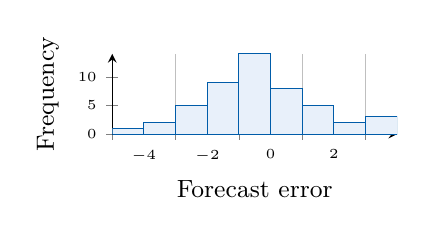
\begin{tikzpicture}
        \begin{axis}[
          width=5.2cm, height=2.6cm,
          ybar interval, bar width=10pt,
          xlabel={\small Forecast error}, ylabel={\small Frequency},
          xmin=-4, xmax=5, ymin=0,
          xtick={-4,-2,0,2,4},
          tick label style={font=\tiny},
          label style={font=\small},
          axis lines=left,
        ]
          \addplot[fill=unolightblue, draw=unoblue]
            coordinates {(-4,1)(-3,2)(-2,5)(-1,9)(0,14)(1,8)(2,5)(3,2)(4,3)(5,0)};
        \end{axis}
      \end{tikzpicture}
    \column{0.46\textwidth}
      \begin{examplebox}{Retail inventory cost}
        {\small Stockout cost $= 5\times$ overstock cost.
        The loss function is \emph{asymmetric} and favors penalizing
        large underestimates.\\[3pt]
        $\Rightarrow$ RMSE aligns better than MAE.\\[3pt]
        $\Rightarrow$ Ideally: use asymmetric loss $L(e) = c_1 e^{+}
        + c_2 e^{-}$, where $e^{+}=\max(e,0)$, $e^{-}=\max(-e,0)$.}
      \end{examplebox}
      \muted{\footnotesize\itshape
        Never report only RMSE --- always show MAE to reveal
        whether accuracy is driven by a few outlier periods.}
  \end{columns}
\end{frame}

% --- Slide: MAPE pitfalls and MASE --------------------------------------------
\begin{frame}{MAPE Pitfalls and When to Use MASE}
  \textbf{MAPE failure cases:}
  \begin{columns}[T]
    \column{0.52\textwidth}
      \begin{itemize}\small
        \item $y_{T+h} \approx 0$ $\Rightarrow$ MAPE $\to \infty$
              (e.g., new product launch, zero-demand months)
        \item \textbf{Asymmetric:} when $y>0$, under-forecasts contribute
              at most 100\% to MAPE (bounded: $\hat{y}=0 \Rightarrow |e/y|=1$);
              over-forecasts are unbounded above
              ($\hat{y}\to\infty \Rightarrow$ MAPE $\to\infty$)
        \item Percentage errors favor low-variance series
      \end{itemize}
    \column{0.44\textwidth}
      \begin{keybox}
        {\small \textbf{MASE} \parencite{Hyndman2006}:\\[2pt]
        $\operatorname{MASE} < 1$ $\Rightarrow$ beats seasonal na\"{i}ve\\
        $\operatorname{MASE} > 1$ $\Rightarrow$ worse than na\"{i}ve\\[2pt]
        Works for intermittent demand, zero values, and cross-series
        comparison.}
      \end{keybox}
  \end{columns}
  \vspace{0.1cm}
  \textbf{Practical recommendation:} report RMSE + MAE for absolute
  accuracy; MASE for benchmarking; MAPE only when $y_t \gg 0$.
  \muted{\footnotesize\itshape
    Socratic: a new product launches in month~1 with $y_1=0$.
    Which metric can you \emph{not} compute, and what do you use instead?}
\end{frame}

% --- Slide: Horizon profiles --------------------------------------------------
\begin{frame}{Accuracy by Horizon}
  \textbf{Key insight:} the winner at $h=1$ is not always the winner at $h=12$.
  \begin{columns}[T]
    \column{0.52\textwidth}
      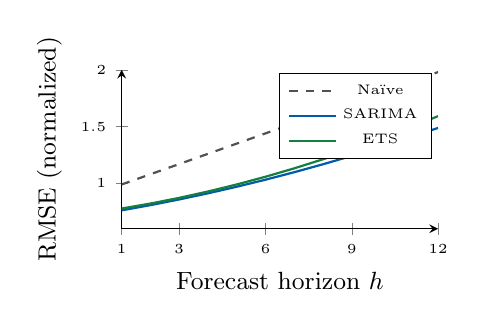
\begin{tikzpicture}
        \begin{axis}[
          width=5.6cm, height=3.6cm,
          xlabel={\small Forecast horizon $h$},
          ylabel={\small RMSE (normalized)},
          xmin=1, xmax=12, ymin=0.6, ymax=2.0,
          xtick={1,3,6,9,12},
          tick label style={font=\tiny},
          label style={font=\small},
          legend style={font=\tiny, at={(0.98,0.98)},
                        anchor=north east},
          axis lines=left,
        ]
          % Naive: grows fast
          \addplot[color=unogray, thick, dashed,
                   domain=1:12, samples=12]
            {0.9 + 0.09*x};
          \addlegendentry{Na\"ive}
          % SARIMA: grows slowly
          \addplot[color=unoblue, thick,
                   domain=1:12, samples=12]
            {0.72 + 0.04*x + 0.002*x^2};
          \addlegendentry{SARIMA}
          % ETS: similar to SARIMA, crosses at h~9
          \addplot[color=unogreen, thick,
                   domain=1:12, samples=12]
            {0.74 + 0.035*x + 0.003*x^2};
          \addlegendentry{ETS}
        \end{axis}
      \end{tikzpicture}
    \column{0.44\textwidth}
      \textbf{\textit{Always report accuracy by horizon, not just
      as a single average.}}
      \vspace{0.15cm}
      \textbf{Why profiles diverge:}
      \begin{itemize}\small
        \item At $h=1$: model captures short-run dynamics
        \item At $h=12$: model must extrapolate seasonal patterns
        \item Na\"{i}ve accumulates error with horizon;
              ARIMA/ETS maintain seasonal anchor
      \end{itemize}
      \muted{\footnotesize\itshape
        Lab 6 plots this profile on RSXFS
        with 36 walk-forward origins.}
  \end{columns}
\end{frame}

% =============================================================================
\section{Walk-Forward Validation}
% =============================================================================

\sectionslide{Walk-Forward Validation}{%
  A single test set gives one data point. Walk-forward gives a distribution.}

% --- Slide: Walk-forward idea -------------------------------------------------
\begin{frame}{The Walk-Forward Idea}
  At each \textbf{forecast origin} $t$: fit model on
  $\{y_1,\ldots,y_t\}$, forecast $\{y_{t+1},\ldots,y_{t+H}\}$.
  \begin{center}
  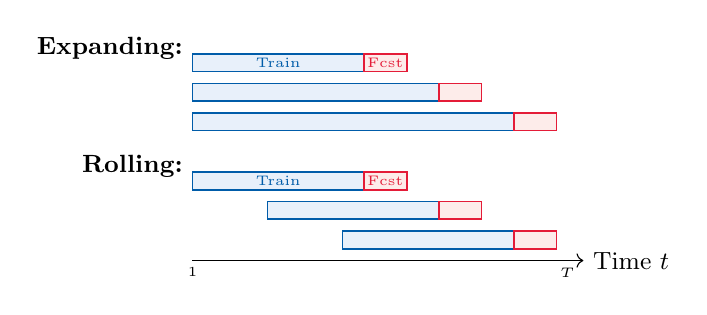
\begin{tikzpicture}[xscale=0.68, yscale=0.75]
    % --- Expanding window ---
    \node[left, font=\small\bfseries] at (0.0, 2.6) {Expanding:};
    \draw[fill=unolightblue, draw=unoblue, line width=0.6pt]
      (0,2.2) rectangle (3.2, 2.5);
    \draw[fill=unolightred, draw=unored, line width=0.6pt]
      (3.2,2.2) rectangle (4.0, 2.5);
    \draw[fill=unolightblue, draw=unoblue, line width=0.6pt]
      (0,1.7) rectangle (4.6, 2.0);
    \draw[fill=unolightred, draw=unored, line width=0.6pt]
      (4.6,1.7) rectangle (5.4, 2.0);
    \draw[fill=unolightblue, draw=unoblue, line width=0.6pt]
      (0,1.2) rectangle (6.0, 1.5);
    \draw[fill=unolightred, draw=unored, line width=0.6pt]
      (6.0,1.2) rectangle (6.8, 1.5);
    \node[font=\tiny, color=unoblue] at (1.6, 2.35) {Train};
    \node[font=\tiny, color=unored]  at (3.6, 2.35) {Fcst};
    % --- Rolling window ---
    \node[left, font=\small\bfseries] at (0.0, 0.6) {Rolling:};
    \draw[fill=unolightblue, draw=unoblue, line width=0.6pt]
      (0.0,0.2) rectangle (3.2, 0.5);
    \draw[fill=unolightred, draw=unored, line width=0.6pt]
      (3.2,0.2) rectangle (4.0, 0.5);
    \draw[fill=unolightblue, draw=unoblue, line width=0.6pt]
      (1.4,-0.3) rectangle (4.6, 0.0);
    \draw[fill=unolightred, draw=unored, line width=0.6pt]
      (4.6,-0.3) rectangle (5.4, 0.0);
    \draw[fill=unolightblue, draw=unoblue, line width=0.6pt]
      (2.8,-0.8) rectangle (6.0, -0.5);
    \draw[fill=unolightred, draw=unored, line width=0.6pt]
      (6.0,-0.8) rectangle (6.8, -0.5);
    \node[font=\tiny, color=unoblue] at (1.6, 0.35) {Train};
    \node[font=\tiny, color=unored]  at (3.6, 0.35) {Fcst};
    % Time axis
    \draw[->] (0,-1.0) -- (7.3,-1.0)
      node[right, font=\small] {Time $t$};
    \node[font=\tiny] at (0,-1.2) {$1$};
    \node[font=\tiny] at (7.0,-1.2) {$T$};
  \end{tikzpicture}
  \end{center}
  \vspace{-0.1cm}
  \muted{\footnotesize\itshape
    \textbf{Expanding:} train grows at each origin.
    \textbf{Rolling:} fixed-size window shifts forward.
    Both produce a time series of forecast errors per horizon $h$.}
\end{frame}

% --- Slide: Rolling vs expanding decision ------------------------------------
\begin{frame}{Rolling vs.\ Expanding: When to Use Which}
  \begin{columns}[T]
    \column{0.50\textwidth}
      \textbf{Use expanding window when:}
      \begin{itemize}\small
        \item Data-generating process is \emph{stable} over time
        \item More training data $\to$ better parameters
        \item Long series with no structural breaks
      \end{itemize}
      \vspace{0.15cm}
      \textbf{Use rolling window when:}
      \begin{itemize}\small
        \item Structural breaks (e.g., COVID-19 shock)
        \item Time-varying parameters / regime change
        \item Fixed window forces model to ``forget'' old patterns
      \end{itemize}
    \column{0.46\textwidth}
      \begin{warningbox}
        {\small \textbf{Minimum training size:} choose $T_0$ large enough
        for reliable estimation. For SARIMA$(p,d,q)(P,D,Q)_m$:
        at least $3m + p + P$ observations.\\[3pt]
        For monthly data: $T_0 \geq 36$ months.}
      \end{warningbox}
      \vspace{0.1cm}
      \textbf{Python:} \texttt{TimeSeriesSplit} in
      \texttt{sklearn.model\_selection}
      implements expanding-window CV; rolling requires a manual loop.
  \end{columns}
\end{frame}

% --- Slide: Walk-forward recipe -----------------------------------------------
\begin{frame}{Walk-Forward Validation: Step-by-Step}
  \begin{columns}[T]
    \column{0.52\textwidth}
      \begin{enumerate}\small
        \item Choose: first origin $T_0$, window type, horizon $H$
        \item \textbf{For} each origin $t = T_0, T_0+1, \ldots, T-H$:
          \begin{enumerate}[(a)]\footnotesize
            \item Fit model on $\{y_1,\ldots,y_t\}$
            \item Generate forecasts $\hat{y}_{t+h|t}$, $h=1,\ldots,H$
            \item Store errors $e_{t,h} = y_{t+h} - \hat{y}_{t+h|t}$
          \end{enumerate}
        \item Average over origins per horizon:
          \[
            \RMSE_h = \sqrt{\tfrac{1}{n_h}\textstyle\sum_t e_{t,h}^2}
          \]
        \item Plot horizon profile; run DM test for significance
      \end{enumerate}
    \column{0.44\textwidth}
      \begin{keybox}
        Walk-forward errors are the closest thing to a \textbf{live
        forecast track record}: each $e_{t,h}$ represents the error
        you would have made if you had used this model in real time.
      \end{keybox}
      \muted{\footnotesize\itshape
        $e_{t,h}$ generalizes $e_{T+h}$ from the Error Metrics section to multiple
        origins~$t$; the metric formulas are the same, averaged over~$t$.\\
        Number of origins $n_h = T - T_0 - H + 1$ for $h=H$;
        with monthly data, 24--36 origins is typical.}
  \end{columns}
\end{frame}

% --- Slide: Walk-forward results table ----------------------------------------
\begin{frame}{Walk-Forward Results: Model Zoo on RSXFS}
  \textbf{Illustrative results} (36 expanding-window origins, $H=12$):
  \begin{center}
    {\footnotesize
    \begin{tabular}{lrrrr}
      \toprule
      \textbf{Model} & \textbf{RMSE$_{h=1}$} & \textbf{RMSE$_{h=3}$}
                     & \textbf{RMSE$_{h=12}$} & \textbf{MASE} \\
      \midrule
      Na\"{i}ve (seasonal)   & 2{,}810 & 3{,}145 & 4{,}210 & 1.00 \\
      SARIMA(1,1,1)(0,1,1)   & 1{,}720 & 2{,}040 & 3{,}480 & 0.76 \\
      ETS (auto-AIC)         & 1{,}690 & 2{,}020 & 3{,}510 & 0.75 \\
      ARIMAX (+ sentiment)   & 1{,}640 & 1{,}980 & 3{,}530 & 0.73 \\
      VAR (BIC order)        & 1{,}660 & 2{,}100 & 3{,}620 & 0.77 \\
      \midrule
      Equal-weight combo     & \textbf{1{,}600} & \textbf{1{,}920}
                             & \textbf{3{,}390} & \textbf{0.71} \\
      \bottomrule
    \end{tabular}
    }
  \end{center}
  \muted{\footnotesize\itshape
    Combination beats all individual models across every horizon.
    Is the ETS vs.\ SARIMA gap statistically real? $\to$ Section 4.}
\end{frame}

% =============================================================================
\section{The Diebold-Mariano Test}
% =============================================================================

\sectionslide{The Diebold-Mariano Test}{%
  Visual inspection says Model A looks better. The DM test asks:
  is the gap statistically real?}

% --- Slide: DM test --- loss differentials ------------------------------------
\begin{frame}{DM Test: Loss Differentials}
  To compare two models, examine the \textbf{loss differential} at each origin.
  \begin{columns}[T]
    \column{0.52\textwidth}
      \begin{definitionbox}{Loss Differential}
        {\small
        For each origin $t$, let:
        \[
          d_t = g(e_{1t}) - g(e_{2t})
        \]
        where $g(\cdot)$ is any loss function.\\[2pt]
        For MSE loss: $d_t = e_{1t}^2 - e_{2t}^2$.\\[4pt]
        Average loss differential:
        \[
          \bar{d} = \tfrac{1}{n}\textstyle\sum_{t=1}^n d_t
        \]
        }
      \end{definitionbox}
    \column{0.44\textwidth}
      \textbf{Numeric example} (MSE loss, $h=1$):\\[4pt]
      {\small
      Origin 1: SARIMA error $= 3.2$, ETS error $= 2.8$\\
      $d_1 = 3.2^2 - 2.8^2 = 10.24 - 7.84 = +2.40$\\[3pt]
      If $\bar{d} > 0$: Model~1 has higher average loss $\Rightarrow$ Model~2 is better.\\[5pt]
      But is $\bar{d}$ statistically distinguishable from~0?\\
      $\to$ \textbf{See next slide.}
      }
  \end{columns}
\end{frame}

% --- Slide: DM test statistic -------------------------------------------------
\begin{frame}{DM Test: The Statistic}
  \begin{definitionbox}{Diebold-Mariano Test \parencite{Diebold1995}}
    {\small
    \[
      DM = \frac{\bar{d}}{\widehat{\operatorname{se}}(\bar{d})}
      \;\xrightarrow{d}\; \mathcal{N}(0,1)
    \]
    \vspace{-3pt}
    {\footnotesize $\bar{d}$: average loss differential (see prev.\ slide);
    $\widehat{\operatorname{se}}(\bar{d})$: HAC standard error.}\\[3pt]
    $H_0$: equal predictive accuracy $\bigl(\E[d_t] = 0\bigr)$.}
  \end{definitionbox}
  \begin{columns}[T]
    \column{0.54\textwidth}
      \textbf{Why HAC?} For an $h$-step forecast, $d_t$ is serially
      correlated up to lag $h-1$ (overlapping forecast errors).
      Ignoring this understates the standard error.
    \column{0.42\textwidth}
      \begin{warningbox}
        {\small Use Newey-West bandwidth $= h-1$ for the HAC
        variance; with $h=1$ (one-step forecasts), $d_t$ is
        white noise under $H_0$.}
      \end{warningbox}
  \end{columns}
\end{frame}

% --- Slide: DM interpretation + loss differential plot -----------------------
\begin{frame}{Interpreting the DM Test}
  \textbf{SARIMA vs.\ ETS on RSXFS} ($h=1$, 36 origins, MSE loss):
  \begin{columns}[T]
    \column{0.56\textwidth}
      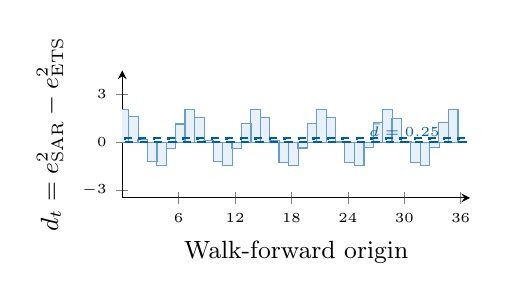
\begin{tikzpicture}
        \begin{axis}[
          ybar, bar width=3.5pt,
          width=6.0cm, height=3.2cm,
          xlabel={\small Walk-forward origin},
          ylabel={\small $d_t = e_{\text{SAR}}^2 - e_{\text{ETS}}^2$},
          xmin=0, xmax=37, ymin=-3.5, ymax=4.5,
          xtick={6,12,18,24,30,36},
          ytick={-3,0,3},
          tick label style={font=\tiny},
          label style={font=\small},
          axis lines=left,
        ]
          \addplot[fill=unolightblue, draw=unoblue!60,
                   samples at={1,...,36}]
            { sin(deg(x*0.9 + 0.5))*1.8 + 0.25 };
          \addplot[color=unoblue, thick, dashed, domain=0:37]
            {0.25};
          \node[font=\tiny, color=unoblue] at (axis cs: 30, 0.75)
            {$\bar{d}=0.25$};
        \end{axis}
      \end{tikzpicture}
    \column{0.40\textwidth}
      \textbf{Decision rule:}
      \begin{itemize}\small
        \item $DM > 1.645$ (one-sided): Model 2 significantly better
        \item $|DM| > 1.96$ (two-sided): models differ significantly
        \item Fail to reject: insufficient evidence --- do not conclude
              models are equal
      \end{itemize}
      \muted{\footnotesize\itshape
        $\bar{d} > 0$: SARIMA has
        slightly higher MSE. If $DM > 1.645$, use ETS.}
  \end{columns}
\end{frame}

% --- Slide: DM caveats --------------------------------------------------------
\begin{frame}{DM Test: Caveats and Extensions}
  \begin{columns}[T]
    \column{0.54\textwidth}
      \textbf{When the DM test applies:}
      \begin{itemize}\small
        \item Non-nested models (e.g., SARIMA vs.\ ETS)
        \item Stationary loss differentials $d_t$
        \item Sufficient number of origins ($n \geq 20$)
      \end{itemize}
      \vspace{0.1cm}
      \textbf{When it does not apply:}
      \begin{itemize}\small
        \item \textbf{Nested models} (e.g., AR(1) vs.\ AR(2)):
              under $H_0$ the DM statistic is non-standard.
              Use the Clark-West correction \parencite{Clark2007}
        \item Very small samples ($n < 15$): use finite-sample
              correction \parencite{Harvey1997}
      \end{itemize}
    \column{0.42\textwidth}
      \begin{keybox}
        {\small DM tests \textbf{equal expected loss}, not model fit.\\[3pt]
        Always use \emph{out-of-sample} walk-forward errors ---
        never in-sample residuals.\\[3pt]
        Always specify the loss function $g(\cdot)$: MSE, MAE,
        or asymmetric loss.}
      \end{keybox}
  \end{columns}
  \muted{\footnotesize\itshape
    Socratic: if $\bar{d} > 0$ but $DM = 0.8$, what conclusion do you draw?
    What would increase power?}
\end{frame}

% =============================================================================
\section{Forecast Combination}
% =============================================================================

\sectionslide{Forecast Combination}{%
  No single model wins every period.
  Combining forecasts diversifies model risk.}

% --- Slide: Combination intuition ---------------------------------------------
\begin{frame}{Why Combine Forecasts?}
  \begin{columns}[T]
    \column{0.54\textwidth}
      \textbf{The portfolio analogy:} diversification reduces portfolio
      variance when assets are imperfectly correlated.
      \[
        \operatorname{Var}\!\left(\tfrac{1}{2}e_1 + \tfrac{1}{2}e_2\right)
        = \tfrac{1}{4}\bigl(\sigma_1^2 + 2\rho\sigma_1\sigma_2 + \sigma_2^2\bigr)
      \]
      If $\rho < 1$: the combined error variance is smaller than
      the average of individual variances.
      \vspace{0.05cm}
      \textbf{Empirical finding:} \textcite{BatesGranger1969} showed
      that weighted combinations \emph{generally} outperform
      the best individual model in empirical comparisons.
    \column{0.42\textwidth}
      \begin{keybox}
        If two models have equal accuracy but
        their errors are \textbf{not perfectly correlated},
        the simple average outperforms either model alone.
      \end{keybox}
      \muted{\footnotesize\itshape
        SARIMA--ETS error correlation $\approx 0.72$ on RSXFS
        $\Rightarrow$ significant gains from combining.}
  \end{columns}
\end{frame}

% --- Slide: Three strategies + the combination puzzle ------------------------
\begin{frame}{Combination Strategies}
  \begin{center}
    {\small
    \begin{tabular}{llll}
      \toprule
      \textbf{Strategy} & \textbf{Formula} & \textbf{Key property}
                        & \textbf{Practical note} \\
      \midrule
      Equal weights
        & $\hat{y}^C = \frac{1}{K}\sum_k \hat{y}^{(k)}$
        & No estimation needed
        & Surprisingly robust \\
      RMSE weights
        & $w_k \propto \RMSE_k^{-1}$
        & Rewards accuracy
        & Simple; no overfitting \\
      OLS weights
        & $\hat{w}$ from regressing $y$ on $\hat{y}^{(k)}$
        & Optimal in theory
        & Prone to overfitting \\
      \bottomrule
    \end{tabular}
    }
  \end{center}
  \begin{columns}[T]
    \column{0.54\textwidth}
      \textbf{The combination puzzle \parencite{Timmermann2006,StockWatson2004}:}
      estimated OLS weights \emph{often underperform} equal weights
      out-of-sample. Three reasons:
      \begin{enumerate}\footnotesize
        \item Estimation error in $\hat{w}$
        \item Model instability / structural breaks
        \item High collinearity among $\hat{y}^{(k)}$
      \end{enumerate}
    \column{0.42\textwidth}
      \begin{warningbox}
        {\small OLS weights can be negative or $>1$.
        Constrain to $w_k \geq 0$, $\sum w_k = 1$
        in practice. Alternatively: shrink toward
        equal weights via ridge.}
      \end{warningbox}
  \end{columns}
\end{frame}

% --- Slide: Combination results + decision rule --------------------------------
\begin{frame}{Combination in Practice}
  \textbf{Extending our walk-forward results (RSXFS, 36 origins):}
  \begin{center}
    {\small
    \begin{tabular}{lrrr}
      \toprule
      \textbf{Method} & \textbf{RMSE ($h=1$)} & \textbf{RMSE ($h=12$)}
                      & \textbf{MASE (avg)} \\
      \midrule
      Best individual (ARIMAX) & 1{,}640 & 3{,}530 & 0.73 \\
      RMSE-weighted combo      & 1{,}620 & 3{,}410 & 0.72 \\
      \textbf{Equal-weight combo} & \textbf{1{,}600} & \textbf{3{,}390}
                                  & \textbf{0.71} \\
      OLS combo (unconstrained)& 1{,}680 & 3{,}580 & 0.76 \\
      \bottomrule
    \end{tabular}
    }
  \end{center}
  \begin{keybox}
    \textbf{Decision rule:} when uncertain about which model to trust,
    \textbf{combine} (equal weights as default). When you have strong
    theoretical or empirical reasons to prefer one model,
    use it alone --- but verify with the DM test.
  \end{keybox}
  \muted{\footnotesize\itshape
    The M4 competition \parencite{Makridakis2020}: top hybrid submissions
    combined diverse methods. Equal-weight ensembles ranked in the
    top 25\% of all 61 participating methods.}
\end{frame}

% =============================================================================
\section{Key Takeaways and Roadmap}
% =============================================================================

\sectionslide{Key Takeaways and Roadmap}{%
  Five evaluation principles --- from metric choice to forecast combination ---
  that apply across the full course.}

% --- Slide: Key Takeaways -----------------------------------------------------
\begin{frame}{Key Takeaways}
  \begin{keybox}
    {\small
    \begin{enumerate}
      \item \textbf{Metric choice is a business decision:} align RMSE/MAE/MASE
            with the cost structure; MAPE fails near zero.
      \item \textbf{Walk-forward validation} gives a distribution of errors
            across origins --- one split is not sufficient.
      \item \textbf{Diebold-Mariano test} determines whether accuracy
            differences are statistically real (use out-of-sample errors,
            HAC standard errors).
      \item \textbf{Nested model comparisons} require the Clark-West correction;
            standard DM is invalid for nested models.
      \item \textbf{Equal-weight combination} typically matches or beats the
            best individual model --- the combination puzzle.
    \end{enumerate}
    }
  \end{keybox}
  \muted{\footnotesize\itshape
    We now have five model families + rigorous evaluation.
    The next step: machine learning for forecasting.}
\end{frame}

% --- Slide: What's Next -------------------------------------------------------
\begin{frame}{What's Next: Machine Learning for Forecasting}
  Classical forecasting is now complete:
  benchmarks $\to$ regression $\to$ ETS $\to$ ARIMA $\to$ multivariate
  $\to$ \textbf{evaluation}.
  \vspace{0.05cm}
  \begin{keybox}
    \textbf{Lecture 7: Machine Learning Introduction} --- bias-variance
    tradeoff, train/validation/test discipline, and how cross-validation
    extends walk-forward ideas to ML models.
  \end{keybox}
  \vspace{0.05cm}
  \begin{center}
    {\small
    \begin{tabular}{lll}
      \toprule
      \textbf{Aspect} & \textbf{Classical forecasting} & \textbf{ML forecasting} \\
      \midrule
      Model structure  & Specified (ARIMA, VAR)    & Learned from data \\
      Assumptions      & Linearity, normality      & Minimal \\
      Overfitting risk & Lower (few parameters)    & High (regularize!) \\
      Evaluation       & Walk-forward; DM test     & Same + CV grid search \\
      \bottomrule
    \end{tabular}
    }
  \end{center}
  \muted{\small \textbf{Lab 6:} walk-forward on RSXFS, DM test (SARIMA vs.\ ETS),
  forecast combination.}
\end{frame}

% --- References ---------------------------------------------------------------
\begin{frame}[allowframebreaks]{References}
  \printbibliography[heading=none]
\end{frame}

\end{document}
